%% Author: Giacomo Minello

% The document class
% \documentclass{report}
% \documentclass{book}
\documentclass[12pt]{article}
 
\usepackage{graphicx}
\graphicspath{ {./figures/} }
\usepackage{wrapfig}
% babel english 
\usepackage[english]{babel}
%allow H on figures
\usepackage{float}
\usepackage[export]{adjustbox}
\usepackage{csquotes}
\usepackage{tikz}
%indent chapters
\usepackage{indentfirst}
\setlength\parindent{0pt}
\usepackage{booktabs}
\setlength{\headheight}{14.5pt}

%allow subfigures
\usepackage{subcaption}
\usepackage{color}
\usepackage{fancyhdr}
\pagestyle{fancy}

\renewcommand{\headrule}{
\textcolor{red}{\hrule}}
\usepackage{wrapfig}
%references done right
\usepackage[
backend=biber,
sorting=none
]{biblatex}
\addbibresource{references/biblio.bib}

% cross-referenced element become links 
\usepackage[hidelinks]{hyperref}

%This will set the options to configure the behaviour of the links within the document. 
%Every parameter must be comma-separated and the syntax must be in the format parameter=value. 
\hypersetup{
    colorlinks=false,
    %linkcolor=black,
    %urlcolor=cyan,
    %pdftitle={PDF title},
    %pdfpagemode=FullScreen
}
\urlstyle{same}
\pagenumbering{gobble}
\setlength{\parskip}{0.5em}
 


\title{SWIFT: \\
RISKS OF FINANCIAL SYSTEMS IN A CYBER ERA\\
\textcolor{red}{\rule[0.1cm]{13cm}{0.1mm}}
\rule[0.5cm]{13.5cm}{0.6mm}}
\author{Giacomo Minello}
\date{March 2020}

\begin{document}
\begin{titlepage}
% create title
\maketitle
\section*{Assignment}
\begin{enumerate}
    \item How were the various banks attacked? Why was the attack on CBB successful? Was it different in the case of other banks?
    \item How did the series of attacks impact on the banks involved and on the SWIFT system?
    \item What type of solutions you could envisage to guarantee the correct working of this critical infrastructure of global financial markets?
\end{enumerate}

\end{titlepage}

% table of content 
\tableofcontents



\newpage

\listoffigures
\listoftables

\newpage
\pagenumbering{arabic}
\section{The attacks}
    \subsection{SWIFT}
    \begin{wrapfigure}{R}{0.2\textwidth}
    \centering
    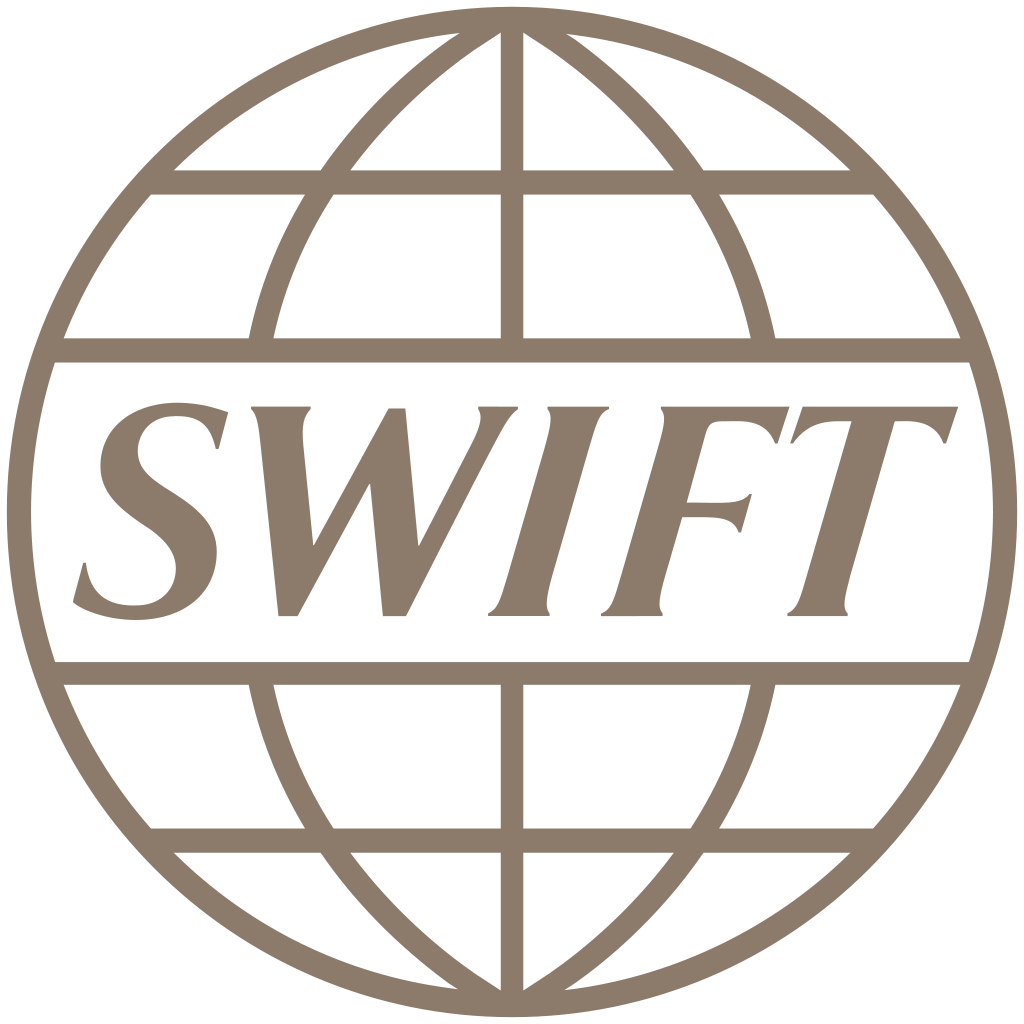
\includegraphics[width=0.15\textwidth]{figures/swiftlogo.png}
    \end{wrapfigure}
        
        SWIFT (the Society for Worldwide Interbank Financial Telecommunications) is a secure messaging service used to transmit financial messages between member institutions around the world. 
        
        SWIFT has served the financial services sector as proprietary communications platform, provider of products and services, standards developer, and conference organizer (Sibos). Founded to create efficiencies by replacing telegram and telex (or “wires”) for international payments, SWIFT now forms a core part of the financial services infrastructure.
    
        SWIFT functions as a member-only cooperative service that is used and trusted by more than 11,000 financial institutions in more than 200 countries and territories around the world.
        
        It is important to clarify that SWIFT is not a payment system but serves as a transport network for a large number of major payment and securities infrastructures. This makes it the most significant provider of global financial messaging and processing services in the world today, a position that its cooperative status is designed to mitigate. The majority of financial institutions use SWIFT to send and receive information about financial transactions. However, SWIFT does not maintain financial information on an ongoing basis and data are only held for a limited period of time. Rather, SWIFT is responsible for providing the network, standards, products, and services that allow member institutions to connect and exchange financial information.
        
        SWIFT distinguishes itself from public Internet Protocol networks by accepting limited liability for defined categories of loss resulting from transaction message delays that have arisen as a consequence of technical issues within SWIFT. Financial service professionals say that the most critical part of SWIFT’s role is achieving the secure exchange of proprietary data – in other words: reliability, confidentiality, and integrity
        
        Although sometimes referred to as not for profit, SWIFT is more accurately committed to being a “not-for-profit maximization” organization. Over the last ten years, SWIFT management have prioritized a reduction in per message costs.
        The cooperative status also imposes certain obligations on members to support SWIFT in kind, through contribution of relevant expertise and an undertaking to route a substantial portion of messaging through SWIFT. However, not all organizations that use the SWIFT network are eligible to be shareholders. SWIFT users are grouped into three categories, each of which has access to different levels of service from SWIFT: supervised financial institutions can send and receive all types of messages; non-supervised entities active in the financial industry can send all type of messages to supervised financial institutions but cannot send or receive payment messages to or from other non-supervised entities; and closed user groups and corporate entities have access to services as defined by the administrator of the closed user group or, for corporate entities, according to criteria defined in the relevant service. Only members of the first category – who are banks, securities broker-dealers, and regulated investment management institutions – would be eligible to be shareholders of SWIFT. 
        
        Management of SWIFT is organized among three groups (marketing, IT operations, and finance and administration) and two functions (legal and human resources), across three regions (Americas, Asia-Pacific, and EMEA). Marketing has a broad brief encompassing product portfolio management, global communication, innovation, and standards. IT operations is not only responsible for the day-to-day running of the SWIFT network but also product development and security control. Finance and administration is responsible for financial management, corporate planning, and pricing of products as well as all internal support functions such as procurement, internal IT, and office management.
        Payments between counterparties are not generally processed instantly, which means that payment systems will often process payments and monetary claims on the basis of “promises to pay”, rather than actual transfer of funds. To facilitate this exchange and guarantee as much as possible the completion of the transaction, payment systems initiate a sequence of events that involves a number of financial institutions and technologies such as banks, clearinghouses, data transmission links, and electronic accounting systems. There are generally three basic stages or processes which are triggered each time a payment needs to be executed, as we can see in table \ref{tab:steptable}.

        % Please add the following required packages to your document preamble:
        % \usepackage{booktabs}
        \begin{table}[H]
        \caption{Description of payment system processes.}
        \label{tab:steptable}
        \begin{tabular}{@{}ll@{}}
        \toprule
        \textit{Payment stage}                                                                             & \textit{Description}                                                                                                                                                                                                                                        \\ \midrule
        \begin{tabular}[c]{@{}l@{}}1. Authorization and initiation of the \\ payment\end{tabular}          & \begin{tabular}[c]{@{}l@{}}This stage involves the submission of\\ the payment order by the payer in\\ order for the funds to be transferred.\end{tabular}                                                                                                  \\
        \begin{tabular}[c]{@{}l@{}}2. Transmission and exchange of the\\ payment instructions\end{tabular} & \begin{tabular}[c]{@{}l@{}}This involves the transmission and\\ exchange of obligations between the\\ parties involved in the transaction.\\ This process may also include the\\ netting (or offsetting) of the\\ obligations where necessary.\end{tabular} \\
        3. Settlement of the payment                                                                       & \begin{tabular}[c]{@{}l@{}}This final stage entails the compensation\\ sent from the payer’s bank to the\\ payee’s bank. A third-party\\ settlement agent is usually involved\\ in this process.\end{tabular}                                               \\ \bottomrule
        \end{tabular}
        \end{table}

        At each step of the payment lifecycle, the payment system must be efficient and reliable in order to avoid any operational and financial risks and ultimately ensure the exchange of funds. Such time-sensitive systems, often referred to as Large-Value Payment Systems (LVPS), usually incorporate real-time gross settlement (RTGS) as part of their payment process. Since the attributes of such systems, and the risks associated, are of great interest to central banks, it is common that they will be actively involved in the governance and decision-making that control these. Quite often central banks will own the domestic LVPSs and operate the various payment and settlement services, though when this is not the case they will monitor operations and oversee any developments while ensuring that the payment systems generally comply with the core principles identified by regulations. Typically, when central banks do not own the system themselves they act as settlement agents within the payment process. 
        
        In the case of cross-border payments, depending on the payment system architecture, the routing of the messages (the second stage of the payment) can take many different forms. The simplest and most popular structure of message flows used by the majority of RTGS systems around the world is the V-shaped structure depicted in figure \ref{fig:vshape}.
        
        \begin{figure}[H]
        \centering
        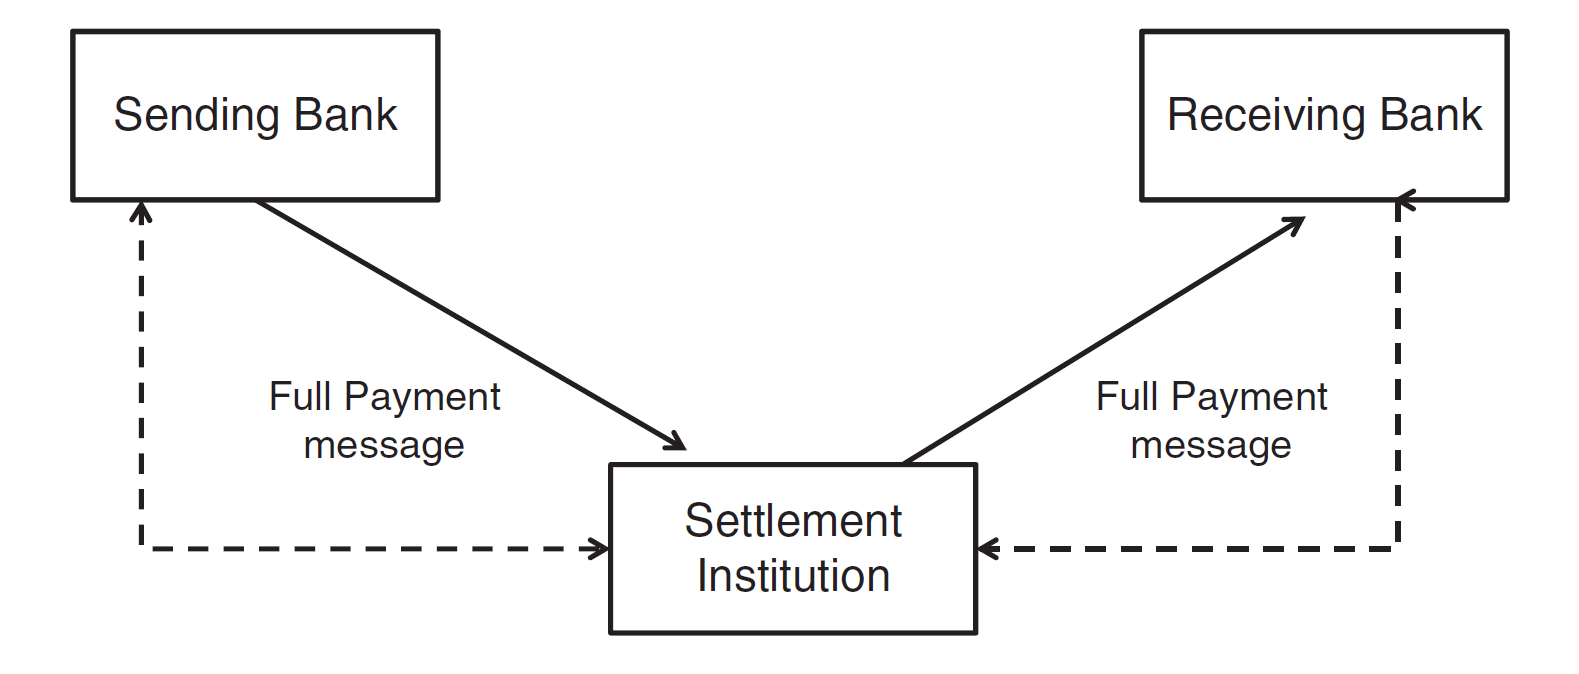
\includegraphics[width=\textwidth]{figures/vshape.png}
        \caption{V-shaped message flow structure.}
        \label{fig:vshape}
        \end{figure}
        
        SWIFT has designed and operates the Y-copy routing, a sophisticated message flow arrangement where SWIFT intercepts the message, copies the entire content of the message, and sends this copy to the settlement institution. Once the SWIFT network receives a respective approval and settlement message from the settlement institution, it forwards the original payment message to the receiving institution as summarized in figure \ref{fig:swiftcloud}.
        
        \begin{figure}[H]
        \centering
        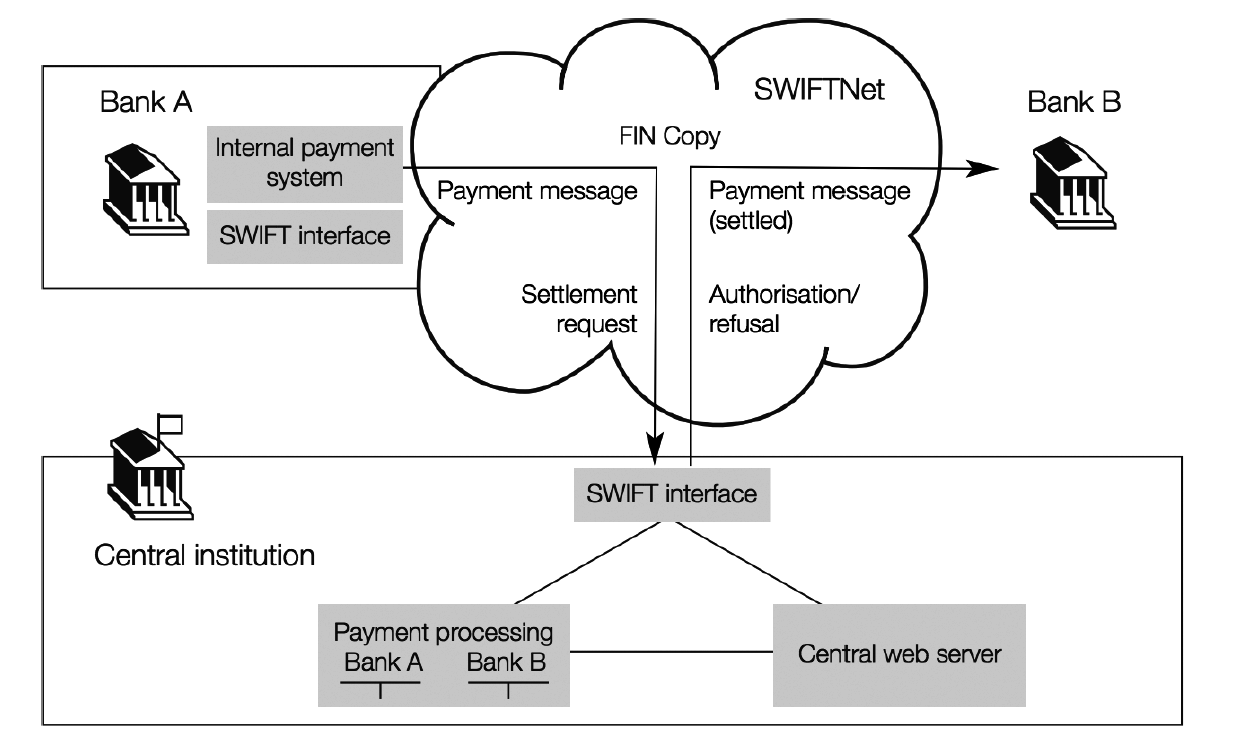
\includegraphics[width=\textwidth]{figures/swiftcloud.png}
        \caption{Y-copy message flow via SWIFTNet.}
        \label{fig:swiftcloud}
        \end{figure}
       
        SWIFT complements the process with a number of query and reporting features that provide users with information useful for their payment operations (e.g. better liquidity management and to achieve reconciliation in case of system outages). Ensuring the integrity of the message is one of the key roles of SWIFT.\cite{scottSocietyWorldwideInterbank2013}
        
        SWIFT does not, however, hold responsibility for the security of its customers’ local SWIFT infrastructure, although it does provide assistance to ensure customers are able to manage cyber attacks. An example of this is the Customer Security Programme (CSP), which was originally introduced in late 2016. A diagram representing how  Full Stack local SWIFT infrastructure model should be secured can be seen in figure \ref{fig:Swift}.
        
        \begin{figure}[H]
        \centering
        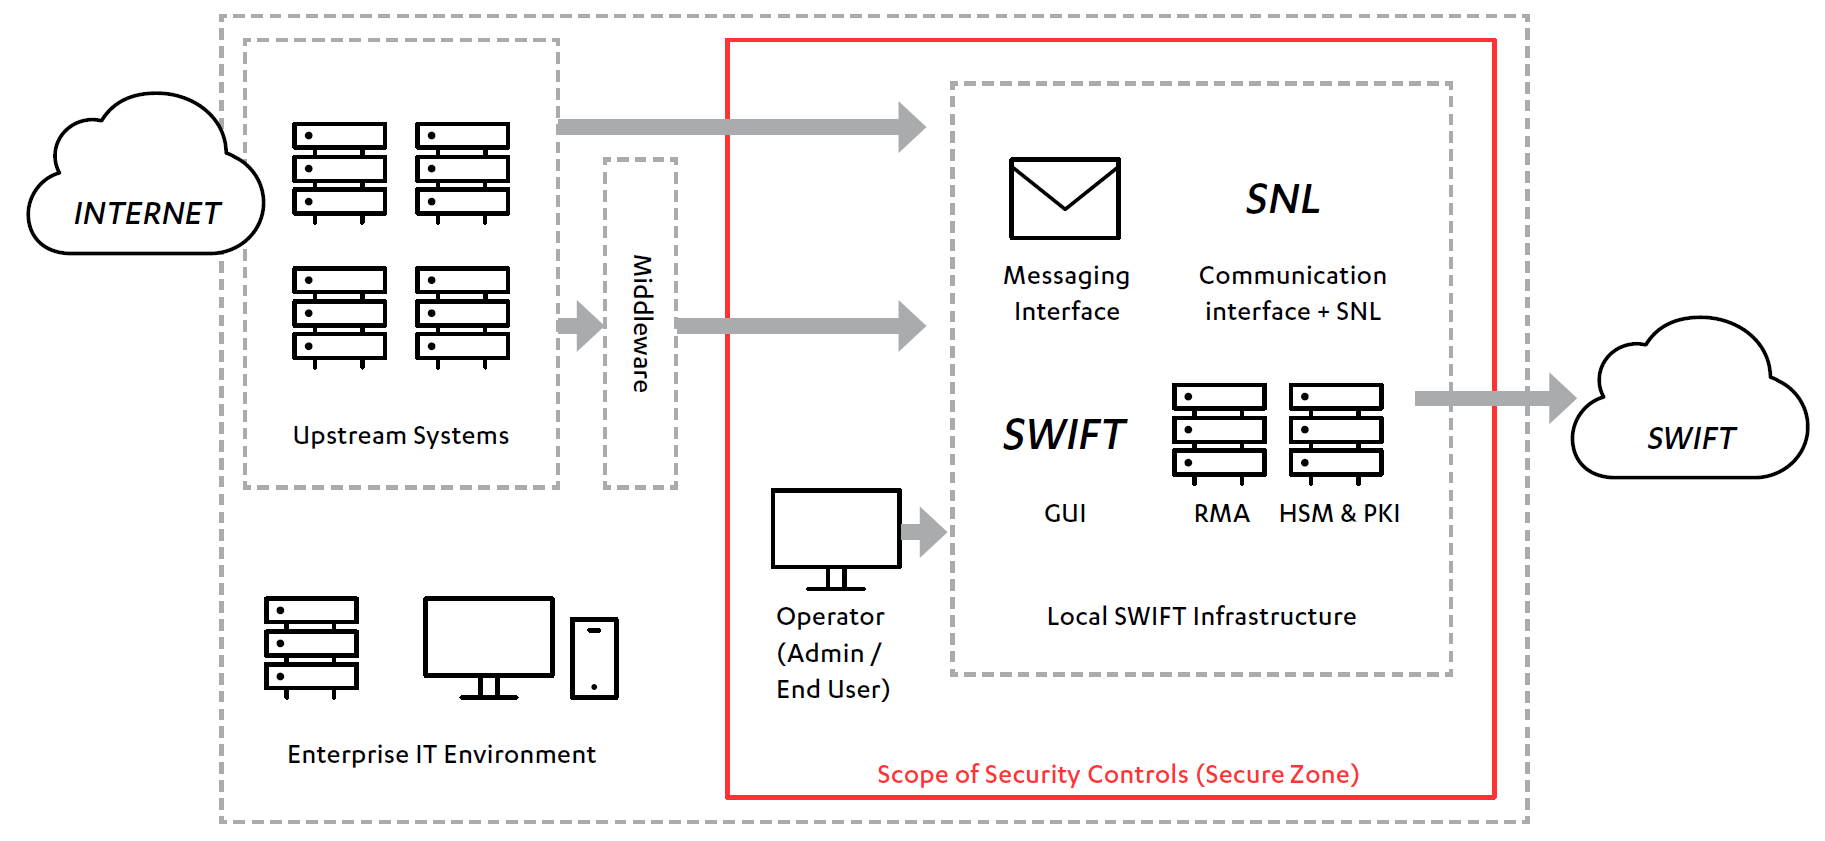
\includegraphics[width=\textwidth]{figures/swift.png}
        \caption{Local SWIFT infrastructure model}
        \label{fig:Swift}
        \end{figure}
        
        The components shown in figure \ref{fig:Swift} are broken down as follows:
        \begin{itemize}
            \item Secure Zone - a segmented portion of the network, isolating SWIFT systems from the rest of the enterprise environment.
            \item Messaging Interface - a software product (e.g. Alliance Access) supporting the use of SWIFT’s messaging services. This is typically connected directly to the Communication Interface.
            \item Communication Interface - a software product (e.g. Alliance Gateway) that provides a link between the SWIFT network (SWIFTNet) and the Messaging Interface software.
            \item  SWIFTNet Link (SNL) - a mandatory software product for access to messaging services over a secure IP network (within the above diagram the SNL is part of the Communication Interface).
            \item HSM & PKI - the SWIFT Hardware Security Module and Public Key Infrastructure.
            \item  RMA - the Relationship Management Application (RMA) is a SWIFT-mandated filter that enables customers to define which counterparties are permitted to send FIN messages to the institution.
            \item Operators -  individual end users and administrators who directly interact with the local SWIFT infrastructure trough computer devices used to operate or maintain the local SWIFT infrastructure.
        \end{itemize}
        
    \subsection{Timeline of high-profile SWIFT-related attacks}
        \begin{figure}[H]
        \centering
        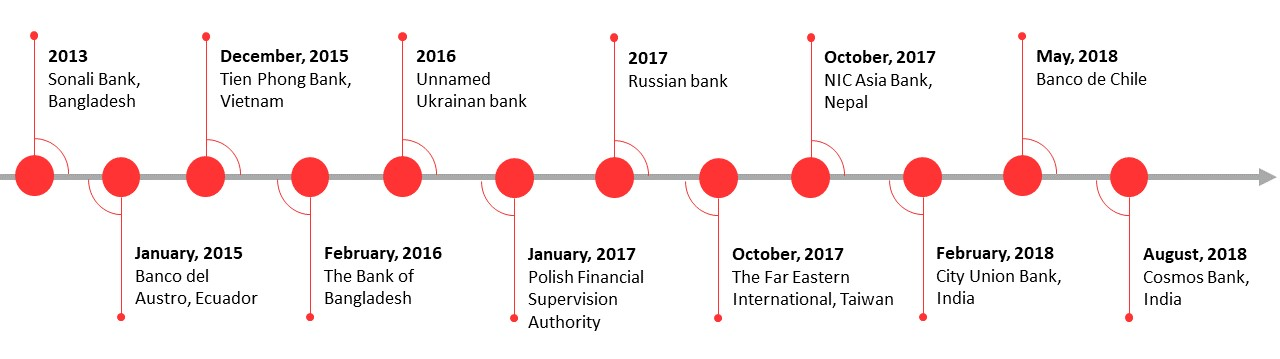
\includegraphics[width=\textwidth]{figures/timelinefinal.jpg}
        \caption{Timeline of the attacks}
        \label{fig:timelineattacks}
        \end{figure}
        
    \subsubsection{Sonali Bank, Bangladesh - 2013}
        Sonali Bank Limited is a state-owned commercial bank in Bangladesh. It is one of the the largest bank of the country.
        
        The unsolved theft of \$250,000 at Sonali Bank involved fraudulent transfer requests sent over the SWIFT international payments network. It is not widely known outside of Bangladesh, and until 2016 it was treated as a ‘cold case’. However, investigators re-opened the case after the attack on the Bank of Bangladesh. 
        
        At Sonali Bank, hackers installed key-logger software on a computer to gain passwords. These credentials were then used to laterally move through the bank’s network in order to gain access to the bank’s internal SWIFT systems; overall \$250,000 worth of SWIFT transactions were made.
        
        Sonali Bank said it had informed SWIFT about the 2013 heist at the time and also unsuccessfully tried to recover the money from the recipients in Turkey.
        
        Police arrested two employees who had responsibility for initiating and approving money transfer instructions, but they were later freed without being charged.\cite{sonali}
        
        \begin{figure}[H]
        \centering
        
\includegraphics[width=\textwidth]{figures/sonali.png}
        \caption{Sonali Bank Hack}
        \label{fig:SonaliHacks}
        \end{figure}
        
    \subsubsection{Banco del Austro, Ecuador - January, 2015}
        The attack, occurred on Jan. 21, 2015, resulted in the theft of \$12.2 million from Banco del Austro, or BDA, in Ecuador. The theft was revealed via a lawsuit filed by BDA against San Francisco-based Wells Fargo. 
        
        The attackers stole the credentials of an unnamed bank employee and used these credentials to access the employee’s Outlook email account. Using this access, the attackers located cancelled and rejected SWIFT transfer requests, altered their details, and reissued them.
        
        In this hack, the transfers were made from Banco del Austro HSBC account in San Francisco to HSBC and Hang Seng Bank accounts in Hong Kong, a Wells Fargo account in Los Angeles, a Mashreqbank account in Dubai, and a JPMorgan Chase account in New York.
        At least \$3.1 million of the funds were then routed from those four companies to 19 “second layer” bank accounts, meaning the funds made a second hop to another set of Hong-Kong registered companies. Most of the “second layer” accounts appeared not to be tied to real businesses and to be controlled by citizens of the People’s Republic of China, according to Hong Kong Deputy High Court Judge Conrad Seagroatt.
        
        BDA discovered that for each unauthorized transfer, an unauthorized user remotely accessed BDA's computer system after hours, logged onto the SWIFT network purporting to be BDA, and redirected transactions to new beneficiaries with significant dollar amounts. 

        BDA's lawsuit blame Wells Fargo for failing to spot the fraud. Each of the unauthorized wire transfers were performed outside normal operating hours of Banco del Austro; it included transactions of significant amounts, which should have triggered an alert at Wells Fargo in their control and verification of the transactions that were being processed.

        BDA also discovered that attackers also attempted to transfer another \$1.4 million from its Citibank accounts to accounts in Dubai and Hong Kong, but those attacks were blocked. The response of Citibank resulted on the immediate refund of the funds.

        Wells Fargo has been blaming BDA's information security policies and procedures for the fraud having occurred and noting that it honored a valid request received via the SWIFT messaging system. For its part, Wells Fargo refunded to BDA \$958,700 out of the \$1,486,230 it transferred to an account in the name of a Jose Mariano Castillo at Wells Fargo in Los Angeles.\cite{AnotherSWIFTHack}\cite{EcuadorBankHacked}\cite{ExclusiveEcuadorCyber2016}\cite{SpecialReportCyber2016}
        
        \begin{figure}[H]
        \centering
        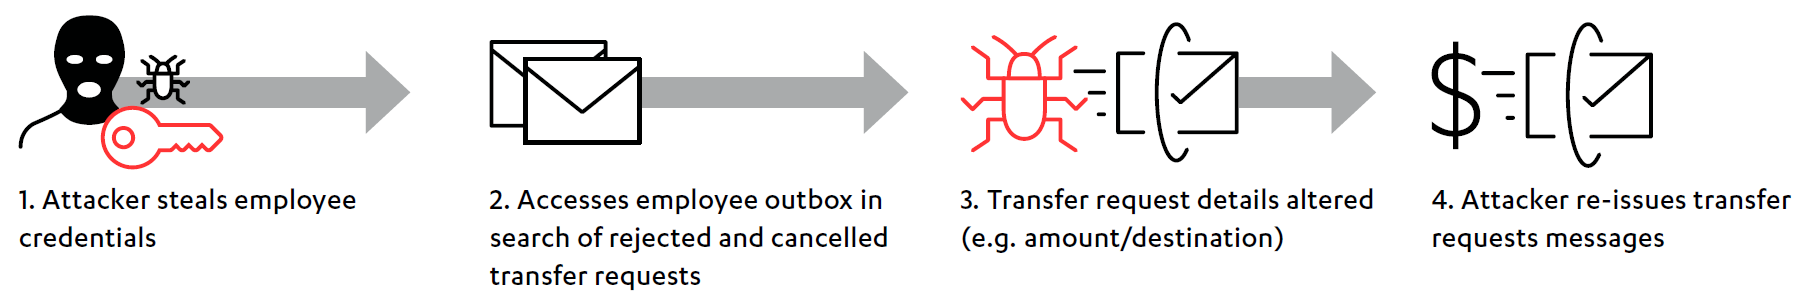
\includegraphics[width=\textwidth]{figures/austro.png}
        \caption{Banco del Austro Hack}
        \label{fig:AustroHacks}
        \end{figure}
        
    \subsubsection{Tien Phong Bank, Vietnam - December, 2015}
    
        Tien Phong Commercial Joint Stock Bank, based in Hanoi, on May 15 said in a statement to Reuters that it detected suspicious transfer requests for \$1.13 million out of its accounts - via the interbank SWIFT messaging system - in the fourth quarter of 2015 as part of a malware attack. The attempted attack did not cause any losses as the bank was quick enough to contact receiving banks and put a stop to the transfers.
        
        The State Bank of Vietnam - the country's central bank – started the investigation on the attack after having received related information from TPBank on May 16.
        
        SWIFT declined to comment on those reports, except to point to a May 13 security alert that it sent to its customers, warning them of "a highly adaptive campaign targeting banks' payment endpoints." That warning said an unnamed Vietnamese bank had been targeted. This led to referring to this attack as an attack towards an “unnamed South-East Asian bank”.\cite{SWIFTWarnsBanks}
        
        TPBank's statement said the fraudulent transfer requests were made using an unnamed third-party vendor with which the bank had contracted, to allow it to interface with the SWIFT network. The bank said that in the wake of the fraudulent transfer requests, it stopped working with the third-party provider and now has a more secure system which directly interfaces with the SWIFT platform.
        
        It was later discovered that the attack against have been carried out using a Trojanized PDF reader. The malware used to target the bank replaces Foxit's PDF reader software,  which was known to be used by the bank employees when viewing SWIFT statements, to mask records of SWIFT transactions when read. When reports are read through the PDF reader, SWIFT records are altered to remove traces of fraudulent transactions.
        
        \begin{figure}[H]
        \centering
        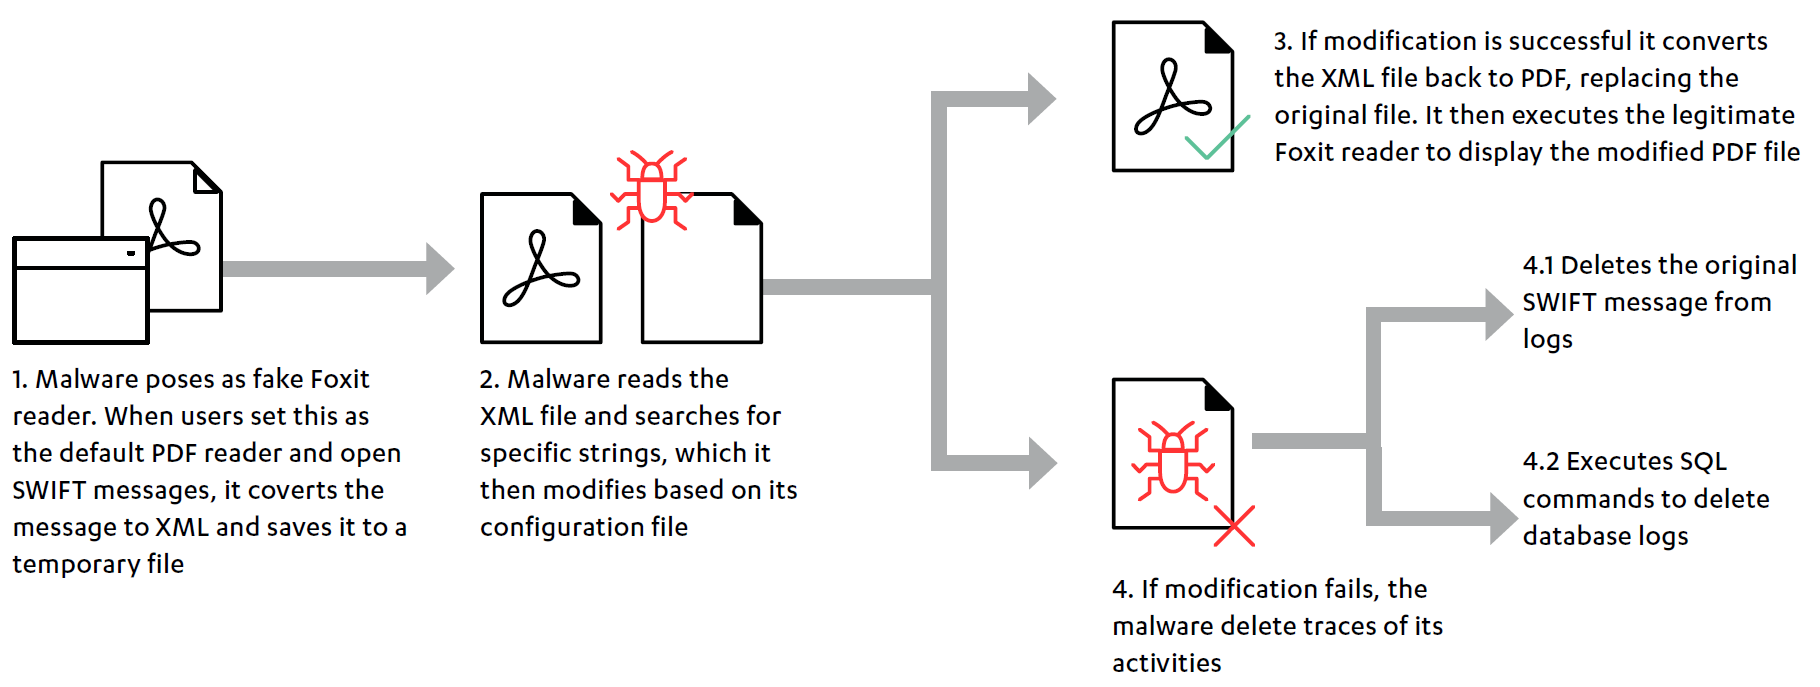
\includegraphics[width=\textwidth]{figures/vietnam.png}
        \caption{Tien Phong Bank Hack}
        \label{fig:VietnamHacks}
        \end{figure}

        Attackers were able to install a malicious version of the Foxit PDF reader on employee workstations, which altered statements (when opened) in order to hide evidence of any malicious activity. This malware was found to be installed on infrastructure provided by a third-party vendor, specifically used to provide the bank’s connection into the SWIFT messaging network, as initially stated by TPBank.
        
        Employees at TPB identified suspicious SWIFT messages in time and contacted all parties involved. This prevented the transfer requests from being completed and the attempt to steal was halted.
        
        BAE Systems stated that it did not have enough evidence to incontrovertibly attribute the hack but it said currently available evidence strongly suggested a connection to the group conducting other similar attacks.\cite{VietnameseBankBlocks}
        
        This attack represent an interesting case due to the months of cooperation between TPB and Kaspersky Lab that uncovered more and more tools hidden deep inside the bank's infrastructure. The second relevant characteristic is the persistence of the attackers: once the contact between that bank and Kaspersky Lab was established, the attackers somehow realized that the behavior of system administrators was not normal and soon after that they started wiping all traces of their activity. However, kaspersky Lab managed to collect and build a rough timeline of some of their operations, as we can see in figure \ref{fig:lazarustimeline}. 
        
        \begin{figure}[H]
        \centering
        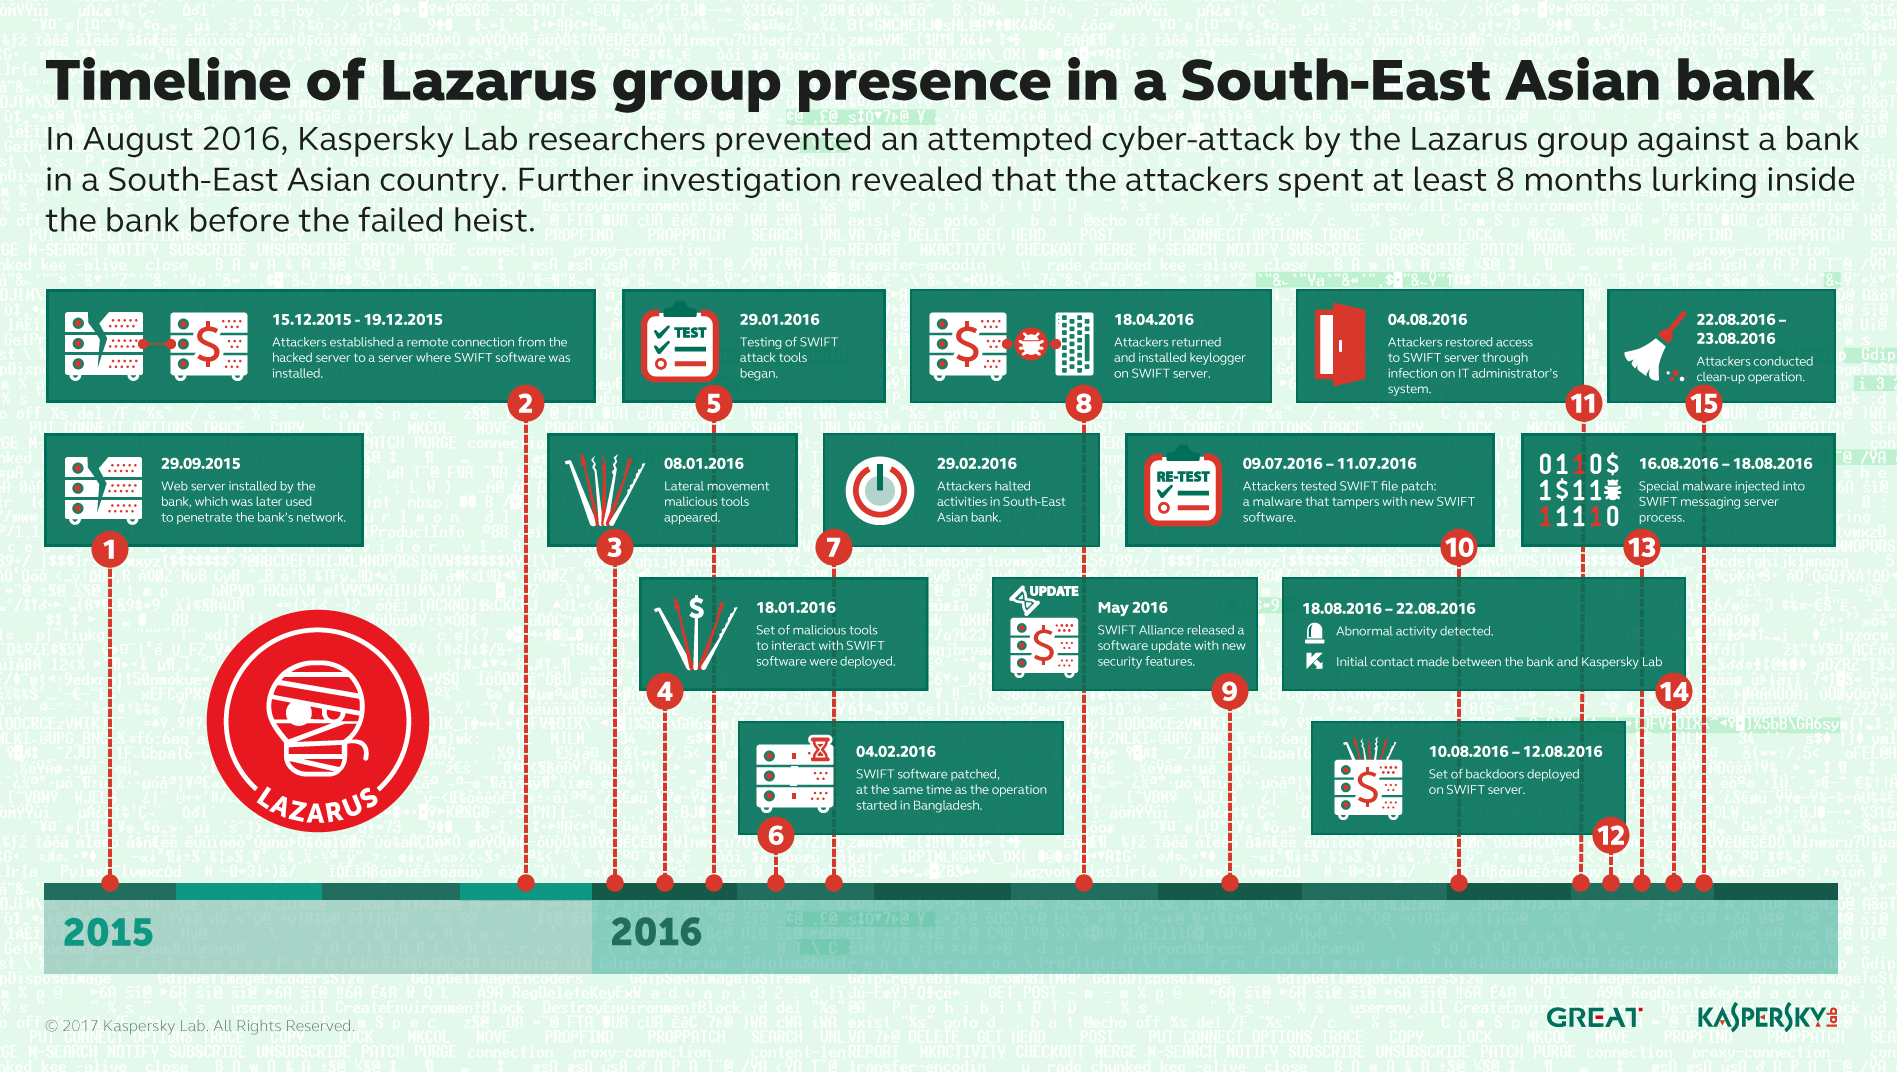
\includegraphics[width=\textwidth]{figures/lazarus-timeline.png}
        \caption{Timeline of the Tien Phong Bank attack according to Kaspersky Lab.}
        \label{fig:lazarustimeline}
        \end{figure}
        
        The investigation suggests attacker activity around 2016-02-04 14:07:07 (UTC) that was also the date of the Bangladesh cyberheist. It was also discovered that the malware used in the two attacks present some visible similarities. 
        
        Due to the age of the breach inside the bank it was not very clear how the attackers initially breached the bank. However, what becomes apparent is that they used a web server located in the bank to connect via Terminal Services to the one linking to SWIFT connected systems.
        
        The web server installation was quite new: it had hosted the company's new website for just a few months before it was compromised. The bank even contracted a pentesting company to do a security assessment of the new website which was ongoing when the attackers breached the server.\cite{kasperskycontenthub}

        Security researcher Christiaan Beek found the code TPBVVNVX - which is the SWIFT code for the Tien Phong Commercial Joint Stock Bank in Hanoi - hidden in multiple parts of the malware used for the attack.
        He also noticed that there were more SWIFT codes in the code:
        \begin{itemize}
            \item UOVBSGSGXXX - United Overseas Bank Ltd, Singapore
            \item ANZBAU3MXXX - Australia and New Zealand Banking Group Ltd, Melbourne, Australia
            \item BOTKJPJTXXX - Bank of Tokyo-Mitsubishi UFJ Ltd, Tokyo, Japan
            \item MHCBJPJTXXX - Mizuho Bank Ltd, Tokyo, Japan
            \item CZNBKRSEXXX - Kookmin Bank, Seoul, South Korea
            \item UNCRITMMXXX - Unicredit S.P.A., Milan, Italy
            \item ICBKVNVNXXX - Industrial and Commercial Bank of China, Hanoi branch, Vietnam
            \item ICBKUS33XXX Industrial and Commercial Bank of China, New York branch, United States
        \end{itemize}
       
         Other than the behaviour above-mentioned, the malware reads the SWIFT messages and checks if the sender of the message is one of the listed banks. Once it finds these messages, it reads their information and then it can manipulate these messages. This information suggest that at a certain point one of the intent of the attack would have involved these potential targets.\cite{AttacksSWIFTBanking2016}
        
    \subsubsection{The Bank of Bangladesh, Bangladesh - February, 2016}
        
        Systems at Bangladesh Bank were infected by "Banswift" malware that allowed attackers to inject fraudulent money-moving messages into the SWIFT network. Attackers also employed trojanized PDF reader software that prevented details of the transactions from being printed out on the bank's printer, thus delaying the bank's discovery of the fraud.
        
        The cyber attack on the Bank of Bangladesh (February 2016) was one of the largest heists and most calculated and sophisticated attacks against SWIFT systems to date. Investigations found that the attack had been patiently executed over the period of almost a full year. Attackers gained access to the bank’s internal systems and deployed trusted Windows software to monitor employee activity. Using this initial foothold, attackers were able to move laterally across the bank’s internal network in search of SWIFT-connected systems. Once access to SWIFT systems was obtained, the attackers monitored employee behaviour, stole user credentials, and deployed specifically-designed malware. The malware targeted the SWIFT Alliance Access application, bypassed its security controls, and removed evidence from printed SWIFT messages.
        In order to grant the ability to execute database transactions, the malware targeted a specific module that was responsible for managing some of the core functions of the database.
        A total of 35 SWIFT transactions worth \$951,000,000 were made. However, only \$81,000,000 of this was successfully exfiltrated to bank accounts in the Philippines, while the rest were blocked and recovered due to typos being identified within a number of SWIFT messages sent.
        
        \begin{figure}[H]
        \centering
        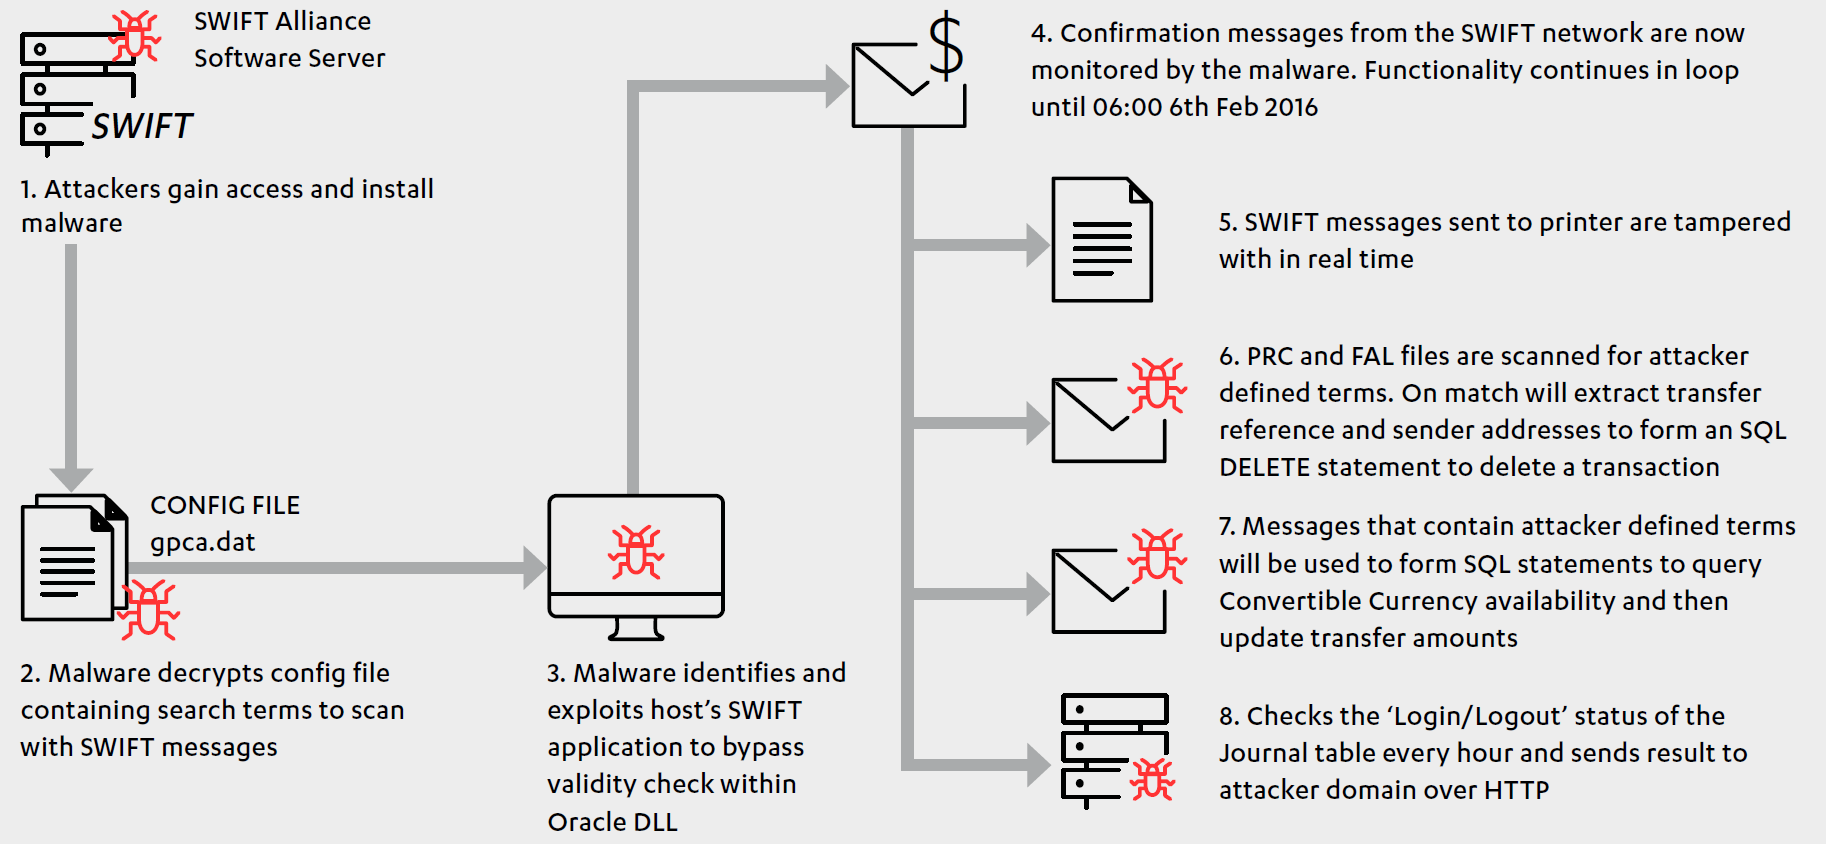
\includegraphics[width=\textwidth]{figures/Bangladesh.png}
        \caption{Bank of Bangladesh Hack}
        \label{fig:Bangladesh}
        \end{figure}
        
        In order to grant the ability to execute database transactions, the malware targeted a specific module that was responsible for managing some of the core functions of the database.
        
        \begin{figure}[H]
        \centering
        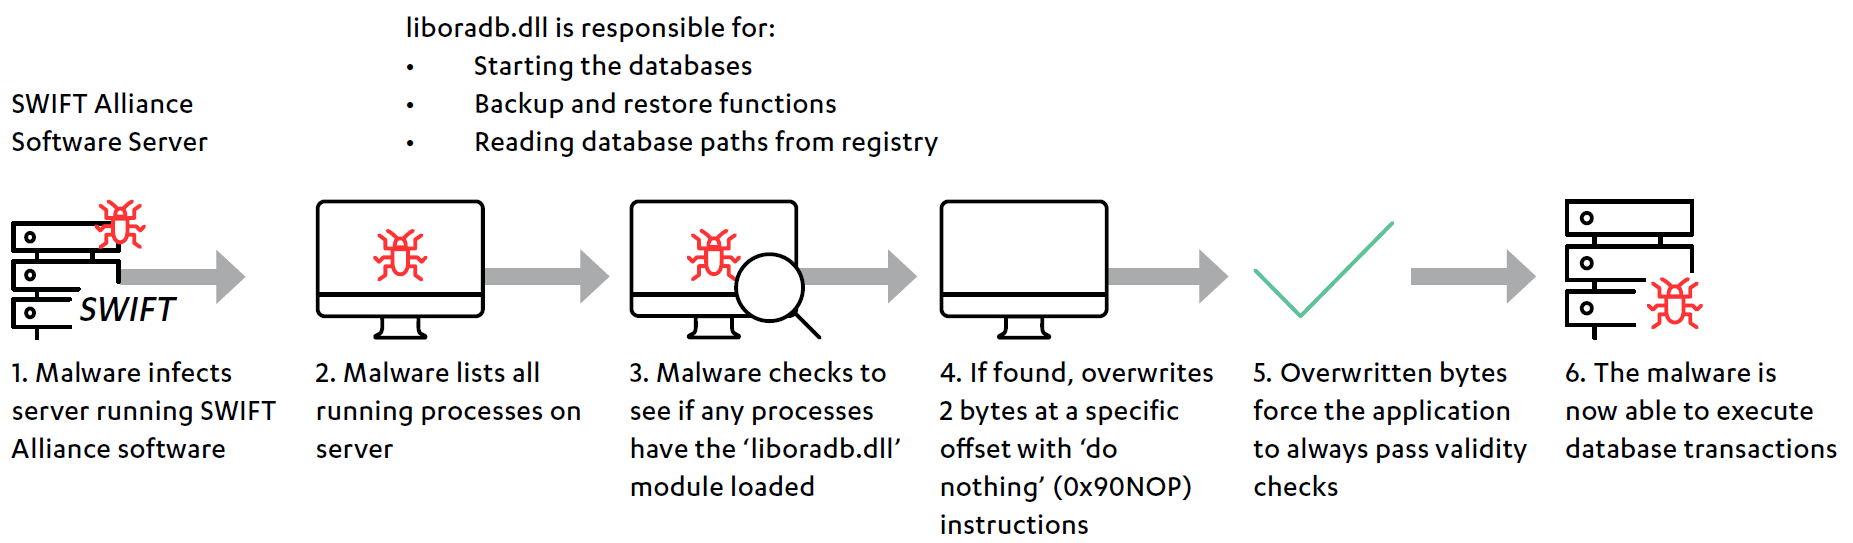
\includegraphics[width=\textwidth]{figures/liboradb.png}
        \caption{How the malware exploited liboradb.dll}
        \label{fig:liboradb}
        \end{figure}
        
        
        https://www.asiapacificsecuritymagazine.com/swift-attackers-malware-linked-to-more-financial-attacks/
        https://outline.com/ZCjsmE
        https://en.m.wikipedia.org/wiki/Bangladesh_Bank_robbery
        https://baesystemsai.blogspot.com/2016/04/two-bytes-to-951m.html
        
    \subsubsection{Unnamed Ukrainan bank - 2016}
        Details regarding the compromise of an unnamed Ukrainian bank are limited, though it was reported that \$10,000,000 was stolen and that the attack was similar to that of the Bank of Bangladesh. 
        
        The Information Systems Audit and Control Association reported that the theft had occurred via the SWIFT system however it did not name which bank had hired some of its members to conduct the investigation.\cite{BangladeshBankEnds}
        
        It was further reported that this attack was only one of many that the Ukraine and Russia had experienced, involving dozens of banks (mostly in Ukraine and Russia), resulting in the loss of “hundreds of millions of dollars”. 
        
        It's not clear if the Ukrainian bank heist involved the same malware or was the work of the same hackers that attacked the Bangladesh Bank as the threat-intelligence firm iSight Partners, a FireEye division, notes that the Ukraine hack may be the work of a different cybercrime organization that used malware to steal an estimated \$25.5 million from Russian bank accounts.\cite{HackersReportedlySteal2016}
   
    \subsubsection{Polish Financial Supervision Authority (Komisja Nadzoru Finansowego) - January, 2017}
        
        In early February 2017, the Polish Financial Supervision Authority (KNF) took its systems offline after discovering that malicious code had been placed on its webserver and was being used to redirect designated targets to malicious payloads. Subsequent public reporting indicates that multiple Polish banks have confirmed that they had identified malware on their systems. Based on further analysis, it is believed that this campaign was more widespread and was intended to primarily target financial institutions.
        
        On Feb. 3, 2017, InfoSec news blog badcyber reported that multiple Polish commercial banks were allegedly infected with malware. The initial investigation suggested that the initial infection vector occurred via the KNF website (figure \ref{fig:knf}). FireEye iSIGHT Intelligence confirmed that unauthorized code was being hosted in a JavaScript file on the KNF domain, which was being used to redirect visitors to an exploit kit landing page. 
        
        \begin{figure}[H]
        \centering
        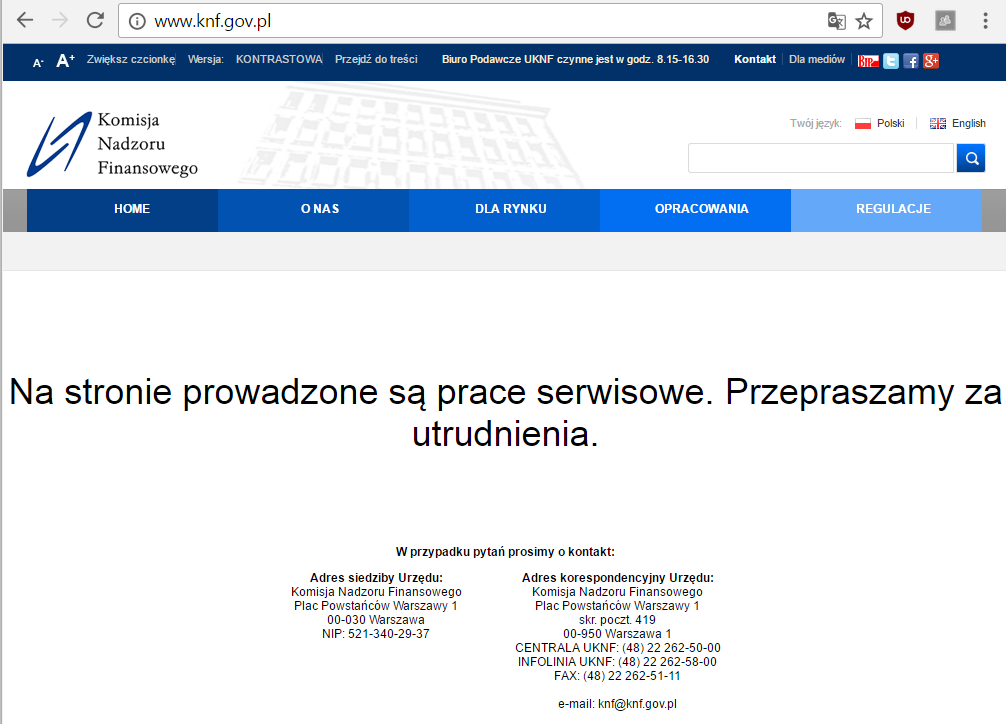
\includegraphics[width=\textwidth]{figures/knf.png}
        \caption{http://www.knf.gov.pl}
        \label{fig:knf}
        \end{figure}
        
        A whitelist of IP addresses observed in conjunction with the KNF incident specified which individuals would receive the designated payload. The whitelist contained IP addresses associated with 104 organizations, many of which are in the financial sector. This whitelist suggests that the threat actors were highly selective in choosing their targets. Most of the whitelisted IP addresses correspond to Polish financial institutions. 
        
        Based on indicators gleaned from open-source reporting, malware associated with the KNF compromise has previously been observed in past SWIFT-related intrusion activity. Given this similarity, it is plausible that KNF intrusion activity shares at least some operational overlap with the SWIFT manipulation attacks widely reported in 2016; however, attribution of this activity is not conclusive.\cite{MungurkApt38}
       
        There is currently no evidence of monetary loss associated with affected Polish banks. However, one media report claimed that a large amount of data was stolen from one Polish financial institution. the nature of the data that was stolen is unclear.\cite{WlamaniaKilkuBankow}\cite{badcyberSeveralPolishBanks2017}\cite{PolishBanksInfected}
    
    \subsubsection{Russian bank - 2017}
        
        The Russian central bank reported the in 2017 unknown hackers stole 339.5 million roubles, roughly \$6 million, from a Russian bank via SWIFT system. 
        
        The hackers had taken control of a computer at a Russian bank and used the SWIFT system to transfer the money to their own accounts. 
        The spokesman of the central bank declined to name the bank or provide further details but he quoted Artem Sychev, deputy head of the central bank’s security department, as saying this was “a common scheme”. In fact, it was reported that during 2016 hackers stole 2 billion rubles from accounts that banks keep at Russia's central bank. During 2016 the attackers tried to steal 5 billion rubles, but the central banking authority managed to stop them and redirect some of the funds. The total loss amounted to 2 billion rubles.
        
        The hackers targeted commercial banks, but they also stole cash from their clients, the central bank reported. At this time, it's unclear who has attacked Russian banks.\cite{HackersStoleMillion2018}\cite{UnknownHackersStole2018}
        
    \subsubsection{The Far Eastern International, Taiwan - October, 2017}
        In October 2017 an attack was carried out against the Far Eastern International Bank. During the heist, attackers used malware which has been linked to multiple attacks on financial institutions around the world. This malware was used to gain access to and move through the bank’s internal network in order to infiltrate SWIFT systems. Attackers then compromised employee credentials and used this information to authenticate to the SWIFT Alliance Messaging Hub and issue a total of \$60,100,000 worth of fraudulent transactions. By the time staff noticed the weird transactions, they had already been wired to banks in the US, Cambodia, and Sri Lanka. Although it was initially understood that \$500,000 was lost, the Financial Supervisory Commission reported that the final amount lost by Far Eastern Bank was \$160,000.\cite{thomsonHackersNick60m2017}
        
        Following an investigation, it was found that the bank’s security posture was not in line with the requirements outlined by Taiwan’s banking law. As a result, Taiwan’s financial regulator fined the Far Eastern International Bank \$266,524, raising the total financial loss of the incident to \$426,524.\cite{TaiwanFarEastern2017}
        
        Also in October, a cyber-security firm BAE Systems Plc said that a North Korean hacking group was likely responsible for a recent cyber heist in Taiwan.\cite{intelligenceBAESystemsThreat}
        
        \begin{figure}[H]
        \centering
        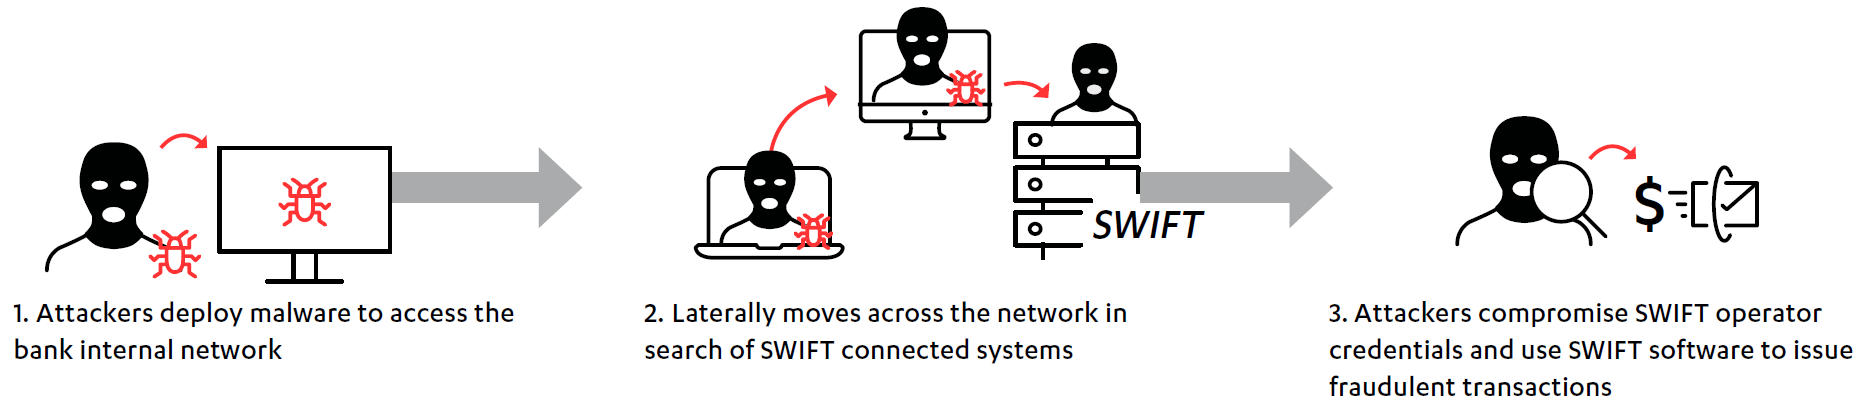
\includegraphics[width=\textwidth]{figures/fareast.png}
        \caption{Far Eastern International Bank Hack}
        \label{fig:FarEastHacks}
        \end{figure}
        
    \subsubsection{NIC Asia Bank, Nepal - October, 2017}
        NIC Asia Bank based in Kathmandu, one of Nepal's largest private-sector commercial banks, said attackers initiated \$4.4 million in fraudulent money transfers through 31 transactions \cite{NICreport} via the SWIFT interbank messaging service from its accounts to accounts in six other countries, including the United States, the United Kingdom, Japan and Singapore, according to the Himalayan News Service. 
        After spotting the suspicious transactions, NIC Asia Bank informed Nepal's central bank, Nepal Rastra Bank, and NRB was able to recover \$3.9 million, although \$580,000 had already been released to overseas bank account.
        The SWIFT system of the Bank was hacked on 18th and 19th of October, during Tihar - aka Deepawali or Diwali - a five-day Hindu festival and one of Nepal's biggest holidays, from October 17 to October 21.
        The hack attack reportedly targeted NIC Asia Bank's Nostro accounts at Standard Chartered New York and Mashreq Bank New York. Banks hold Nostro accounts at another bank and in a foreign currency to facilitate foreign exchange transactions and trades.
        Roshan Kumar Neupane, deputy CEO at NIC Asia Bank, told PTI news agency that the bank took its SWIFT server offline immediately after spotting the suspicious transactions. After the transactions were discovered, NIC Asia Bank also commissioned KPMG India to conduct a digital forensic review, which it has shared with both NRB and Nepal Police's Central Investigation Bureau. But the results of the investigation reportedly failed to conclude if the theft resulted from an outside attacker or insider theft.
        An investigation into the heist launched by Nepal's central bank found that six staffers in NIC Asia Bank's SWIFT department had used a computer that was meant to be used only for SWIFT transactions for other purposes as well.\cite{ReportAttackersHacked}\cite{NICAsiaBank2017}
        
        
    \subsubsection{City Union Bank, India -  February, 2018}
        
        On Sunday, February 18, the Indian bank Kumbakonam-based City Union Bank announced that cyber criminals compromised its systems and transferred a total of \$1.8 million.  
        
        The Indian bank confirmed that it has suffered a security breach launched international cyber-criminals and there is no evidence of internal staff involvement. 
        
        During the reconciliation process on February 7, it was found out that 3 fraudulent remittances had gone through our SWIFT system to corespondent banks which were not initiated from the bank. The operators immediately alerted the correspondent banks to recall the funds.

        One transaction of \$500,000 that was made through Standard Chartered Bank, New York, to a Dubai based bank was immediately blocked. A second transfer of 300,000 euros (\$372,150) was routed through a Standard Chartered Bank account in Frankfurt to a Turkish account, although the Turkish lender had blocked the transfer from being finalised. A third totaling \$1 million was sent through a Bank of America account in New York to a China-based bank identified as Zhejiang Rural Credit Cooperative Union in Hangzhou, China.\cite{CityUnionBank2018}\cite{IndiaCityUnion2018}

        
    \subsubsection{Banco de Chile - May, 2018}
        
        Banco de Chile, the country's second largest bank, on May 24 lost about \$10 million due to fraudulent SWIFT wire transfers. The theft happened while the bank was dealing with hundreds of workstations and servers that suddenly stopped working.
        
        Researchers with business risk intelligence firm Flashpoint say they've analyzed the malware used for the distraction portion of the attack against Banco de Chile. It's MBR Killer, a component of Buhtrap, a malware a-la NotPetya that first struck Russian banks in 2015. Buhtrap is a portmanteau of the Russian word "buhfalter" that means accountant, and trap. MBR Killer tampers with the master boot record, the first sector of a hard drive that the computer calls on before loading the operating system. The component renders the local operating system and MBR unreadable. The source code for Buhtrap leaked in early 2016, that means any group could be using it now to cause havoc. According to a screenshot of private IM conversations posted on a Chilean forum, the alleged "virus" crashed over 9,000 computers and over 500 servers. This malware didn't bother showing a ransom note and just wiped computer's MBRs, leaving them in a non-bootable state.
        
        Banco de Chile General Manager Eduaro Ebensperger Orrego told the publication Latercera that it was eventually determined the initial attacks were likely a distraction. The real target was the bank's SWIFT system. The bank was able to stop some of the fraudulent transactions. 
        
        The attribution behind the Banco de Chile attack remains uncertain.
        “It is notable, however, that Chilean financial institutions were targeted entities by the Lazarus Group, which was linked to North Korea, during the compromise of the Polish Financial Supervision Authority website in 2017,” Vitali Kremez, director of research, told Threatpost in an interview. 

        \cite{HackersCrashedBank}\cite{BancoChileWiper}\cite{BancoChileLoses}
        
    \subsubsection{Cosmos Bank, India - August, 2018}
        Cosmos Bank is a 112-year old cooperative bank in India and it is the second largest in the country. Between August 10 and 13, 2018, over \$13.5 million were stolen with an attack using multiple techniques, targeting both ATMs and the SWIFT environment. 
        
        On August 11, 2018, the bank’s internal and ATM infrastructure was compromised. The exploit involved multiple malware leveraging a set of malicious libraries with a malicious ATM/POS switch in parallel with the existing Central and then selectively breaking the connection between the Central and the Core Banking System. The use of the malicious switch allowed the attackers to execute ATM withdrawals for over \$11.5 million in 2849 domestic  and 12000 international transactions using 450 cloned debit cards in 28 countries.
        
        On August 13, 2018, the malicious threat actor continued the attack against Cosmos Bank by using the Cosmos bank’s SWIFT credentials to successfully send three malicious transaction to ALM Trading Limited at Hang Seng Bank in Hong Kong amounting to around \$2 million.\cite{CosmosBankSWIFT2018}\cite{PoliceInvestigateCosmos}
        
    \subsubsection*{Other attacks}
        
        https://www.reuters.com/article/us-russia-cyber-globex/russias-globex-bank-says-hackers-targeted-its-swift-computers-idUSKBN1EF294 
        https://www.bankinfosecurity.com/hackers-target-swift-using-banks-odinaff-malware-a-9451
        https://www.pindrop.com/blog/theres-another-hacking-team-going-after-swift-banks/
        https://www.bloomberg.com/news/articles/2018-05-29/mexico-foiled-a-110-million-bank-heist-then-kept-it-a-secret
        https://www.wired.com/story/mexico-bank-hack/
    
    \subsection{The attackers - APT38 a.k.a. Lazarus Group}
        
        \begin{wrapfigure}{R}{0.2\textwidth}
        \centering
        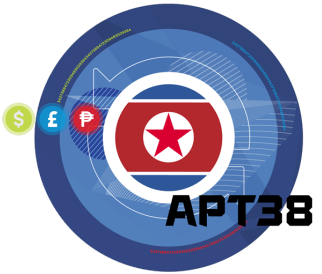
\includegraphics[width=0.20\textwidth]{figures/apt38.png}
        \end{wrapfigure}
        North Korean group definitions are known to have significant overlap, and the name Lazarus Group is known to encompass a broad range of activity. Some organizations use the name Lazarus Group to refer to any activity attributed to North Korea. Some organizations track North Korean clusters or groups such as Bluenoroff, APT37, and APT38 separately, while other organizations may track some activity associated with those group names by the name Lazarus Group.
        
        \begin{figure}[H]
        \centering
        \includegraphics[width=\textwidth]{figures/TESTSwiftHacks.png}
        \caption{Swift Hacks}
        \label{fig:SwiftHacks}
        \end{figure}
        
        https://github.com/mungurk/apt_38/blob/master/HP%20-%20Profiling%20an%20enigma%20-%20Mystery%20of%20North%20Korea's%20Threat%20Landscape.pdf
        
        https://www.youtube.com/watch?v=9Vh2n6nC0t4&feature=emb_title
        
        https://blog.lexfo.fr/ressources/Lexfo-WhitePaper-The_Lazarus_Constellation.pdf
        
        https://www.kaspersky.com/about/press-releases/2017_chasing-lazarus-a-hunt-for-the-infamous-hackers-to-prevent-large-bank-robberies
        
        https://media.kasperskycontenthub.com/wp-content/uploads/sites/43/2018/03/07180244/Lazarus_Under_The_Hood_PDF_final.pdf
        
        https://www.fireeye.com/blog/threat-research/2018/10/apt38-details-on-new-north-korean-regime-backed-threat-group.html
        
        https://baesystemsai.blogspot.com/2016/04/two-bytes-to-951m.html
        
        https://github.com/mungurk/apt_38
        
        https://www.blackhat.com/docs/eu-17/materials/eu-17-Shen-Nation-State%20Moneymules-Hunting-Season-APT-Attacks-Targeting-Financial-Institutions.pdf
        
        https://baesystemsai.blogspot.com/2016/05/cyber-heist-attribution.html
        
\section{The consequences}
        
        As a countermeasure to the current cyber-threat landscape, SWIFT has implemented the Customer Security Programme (CSP). This programme requires all SWIFT customers to implement a number of controls defined by SWIFT’s Customer Security Controls Framework (CSCF), to which customers must self-attest compliance before 1 January 2018. This framework outlines a collection of security controls to ensure a minimal baseline for security is in place across all customers’ local SWIFT deployments.
        
        https://www.justice.gov/opa/press-release/file/1092091/download
        https://en.wikipedia.org/wiki/2015%E2%80%932016_SWIFT_banking_hack
        https://thefinancialexpress.com.bd/trade/reserves-heist-swift-turns-to-govt-seeks-unfettered-staff-travel-1580101565
        https://www.bankinfosecurity.com/security-investments-consume-swifts-profits-a-9988
        
\section{The solutions}
        
        As a countermeasure to the current cyber-threat landscape, SWIFT introduced the Customer Security Program (CSP) to support SWIFT customers in securing their local SWIFT infrastructure. This program requires that all customers implement a set of mandatory and advisory security controls outlined within SWIFT’s Customer Security Controls Framework (CSCF).
        
        These controls have been identified by SWIFT based on cyber-threat intelligence and in collaboration with industry experts, and are articulated around three main objectives:
        1. Secure Your Environment 
        2. Know and Limit Access 
        3. Detect and Respond
        
        https://www.bankinfosecurity.asia/swift-hack-lessons-for-india-a-9095
        

\begin{flushright}
\begin{tikzpicture}
    \node[inner sep=0] (image) at (0,0) {
\includegraphics[width=0.26\textwidth]{figures/firmaMinello.png}};
    \node[below=2cm of image] {Giacomo Minello};
 \end{tikzpicture}
 \end{flushright}
% print biblio with heading in the index
\newpage
\printbibliography[heading=bibintoc]
\end{document}